%Dokumentklasse

%draft als optionohne bilder für bessere performance
%\documentclass[a4paper,12pt,draft]{scrreprt}

%normal mit Bildern
\documentclass[a4paper,12pt]{scrreprt}

\usepackage[left= 3cm,right = 3cm, bottom = 3cm,top = 3cm]{geometry}
%\usepackage[onehalfspacing]{setspace}

% ============= Packages =============

% Dokumentinformationen
\usepackage[
	pdftitle={Praktikum - Umwelttechnik},
	pdfsubject={},
	pdfauthor={Roman-Luca Zank},
	pdfkeywords={},	
	%Links nicht einrahmen
	hidelinks
]{hyperref}

%nur Text zum prüfen des Umfangs

% Standard Packages
\usepackage[utf8]{inputenc}
\usepackage[ngerman]{babel}
\usepackage[T1]{fontenc}

%\usepackage{helvet}
%\renewcommand{\familydefault}{\sfdefault} 

\usepackage{graphicx}
\usepackage{cancel}
\graphicspath{{img/}}
\usepackage{fancyhdr}
\usepackage{lmodern}
\usepackage{color}
\usepackage{placeins}
\usepackage{booktabs}
\usepackage{caption}
\usepackage[list=true]{subcaption}

%Einheitenpackage
\usepackage{siunitx}  
\sisetup{	locale = DE, 
			per-mode=fraction,
			inter-unit-product=\ensuremath{\cdot},
			detect-weight = true,
			quotient-mode=fraction
		}
%neue Einheiten definieren
\DeclareSIUnit\xyz{xyz}		

%Automatisch cdot statt *
\DeclareMathSymbol{*}{\mathbin}{symbols}{"01}



%\setcounter{lofdepth}{2}      %für subfigures in list of figures

%Tabelle
\usepackage{tabularx}
\usepackage{tabulary}

%%Verzeichnispackages
%\usepackage{natbib}

%\usepackage{hyperref}
%\newcites{

% zusätzliche Schriftzeichen der American Mathematical Society
\usepackage{amsfonts}
\usepackage{amsmath}

%Abkürzungsverzeichnis
\usepackage{acronym}

%kein Abstand bei neuem Kapitel vom Seitenanfang
%\vspace*{2.3\baselineskip} = ORIGINAL
\renewcommand*{\chapterheadstartvskip}{\vspace*{.0\baselineskip}}

%nicht einrücken nach Absatz
\setlength{\parindent}{0pt}

% ============= Kopf- und Fußzeile =============
\pagestyle{fancy}
%
\lhead{}
\chead{}
\rhead{}%\slshape }%\leftmark}
%%
\lfoot{}
\cfoot{}
\rfoot{\pagemark}
%%
\renewcommand{\headrulewidth}{0pt}
\renewcommand{\footrulewidth}{0pt}
\renewcommand{\chapterpagestyle}{fancy}

% ============= Package Einstellungen & Sonstiges ============= 
%Besondere Trennungen
%\hyphenation{De-zi-mal-tren-nung}
\usepackage[none]{hyphenat}
\hyphenpenalty=5000
\tolerance=5000
\providecommand\phantomsection{}

\usepackage{mathtools}

% ============= Dokumentbeginn =============

\begin{document}
%Seiten ohne Kopf- und Fußzeile sowie Seitenzahl
\pagestyle{empty}

%\begin{center}
\begin{tabular}{p{\textwidth}}


\begin{center}

\includegraphics[scale=0.75]{img/logos.jpg}\\
\end{center}


\\

\begin{center}
\LARGE{\textsc{
Protokoll \\
Umwelttechnik\\
}}
\end{center}

\\

%\begin{center}
%\large{Fakultät für Muster und Beispiele \\
%der Hochschule Musterhausen \\}
%\end{center}
%
%\\

\begin{center}
\textbf{\Large{V4 - Bodencharakterisierung}}
\end{center}

\begin{center}
	\large{Gruppe 1.2 (BCUT3)}
\end{center}


\\
%\begin{center}
%zur Erlangung des akademischen Grades\\
%Bachelor of Engineering
%\end{center}


%\begin{center}
%vorgelegt von
%\end{center}

\begin{center}
\Large{\textbf{Teilnehmer:}} \\ 
\end{center}
\begin{center}
\large{Willy Messerschmidt \\
		Roman-Luca Zank} \\
\end{center}


\\

\begin{center}
\begin{tabular}{lll}
\large{\textbf{Protokollführer:}} & & \large{Roman oder Willy} \\
& & email@stud.hs-merseburg.de\\
&&\\
\large{\textbf{Datum der Versuchsdurchführung:}}&& \large{12.12.2019}\\
&&\\
\large{\textbf{Abgabedatum:}}&& \large{12.12.2019}
\end{tabular}
\end{center}

\\ \\ \\ \\ \\ \\ \\ 
\large{Merseburg den \today}

\end{tabular}
\end{center}


%\include{14_danksagungen}

%\include{15_zusammenfassung}

% Beendet eine Seite und erzwingt auf den nachfolgenden Seiten die Ausgabe aller Gleitobjekte (z.B. Abbildungen), die bislang definiert, aber noch nicht ausgegeben wurden. Dieser Befehl fügt, falls nötig, eine leere Seite ein, sodaß die nächste Seite nach den Gleitobjekten eine ungerade Seitennummer hat. 
\cleardoubleoddpage

% Pagestyle für Titelblatt leer
\pagestyle{empty}

%Seite zählen ab
\setcounter{page}{0}

%Titelblatt
%\begin{center}
\begin{tabular}{p{\textwidth}}


\begin{center}

\includegraphics[scale=0.75]{img/logos.jpg}\\
\end{center}


\\

\begin{center}
\LARGE{\textsc{
Protokoll \\
Umwelttechnik\\
}}
\end{center}

\\

%\begin{center}
%\large{Fakultät für Muster und Beispiele \\
%der Hochschule Musterhausen \\}
%\end{center}
%
%\\

\begin{center}
\textbf{\Large{V4 - Bodencharakterisierung}}
\end{center}

\begin{center}
	\large{Gruppe 1.2 (BCUT3)}
\end{center}


\\
%\begin{center}
%zur Erlangung des akademischen Grades\\
%Bachelor of Engineering
%\end{center}


%\begin{center}
%vorgelegt von
%\end{center}

\begin{center}
\Large{\textbf{Teilnehmer:}} \\ 
\end{center}
\begin{center}
\large{Willy Messerschmidt \\
		Roman-Luca Zank} \\
\end{center}


\\

\begin{center}
\begin{tabular}{lll}
\large{\textbf{Protokollführer:}} & & \large{Roman oder Willy} \\
& & email@stud.hs-merseburg.de\\
&&\\
\large{\textbf{Datum der Versuchsdurchführung:}}&& \large{12.12.2019}\\
&&\\
\large{\textbf{Abgabedatum:}}&& \large{12.12.2019}
\end{tabular}
\end{center}

\\ \\ \\ \\ \\ \\ \\ 
\large{Merseburg den \today}

\end{tabular}
\end{center}
 %Prokolle
\begin{center}
\begin{tabular}{p{\textwidth}}


\begin{center}

\includegraphics[scale=0.75]{img/logos.jpg}\\
\end{center}


\\

\begin{center}
\LARGE{\textsc{
Mechanische Verfahrenstechnik\\
}}
\end{center}

%\begin{center}
%\large{Fakultät für Muster und Beispiele \\
%der Hochschule Musterhausen \\}
%\end{center}
%
%\\
 \\
 
\begin{center}
\textbf{\Large{Skriptaufzeichnungen}}
\end{center}

\begin{center}
	\large{im WiSe 2019}
\end{center}
 \\
%\begin{center}
%zur Erlangung des akademischen Grades\\
%Bachelor of Engineering
%\end{center}


\begin{center}
\large{vorgelegt von}
\end{center}
\\


\begin{center}
\Large{\textbf{Roman-Luca Zank}} \\
\end{center}

\begin{center}
3. Semester \\
Chemie- und Umwelttechnik \\
\end{center}


\begin{center}
\begin{tabular}{lll}
	\textbf{E-Mail:} & & romanzank@mail.de\\
	\textbf{Matrikelnummer:} & &25240\\
	\textbf{Adresse:} & &Platz der Bausoldaten 2, Zimmer 224\\
	\textbf{Ort:} & &06217 Merseburg\\
	&& \\
	\textbf{Professor:} & & Dr.-Ing. Thomas Martin\\
\end{tabular}
\end{center}

\\ \\ \\ \\ \\
\large{Merseburg, \today}

\end{tabular}
\end{center}
 %Seminar-/Abschlussarbeit

% Pagestyle für Rest des Dokuments
\pagestyle{fancy}

%Inhaltsverzeichnis
\tableofcontents

%Inhalt
%%Verzeichnis aller Bilder
%\label{sec:bilder}
%\listoffigures
%\addcontentsline{toc}{chapter}{Abbildungsverzeichnis}

%Verzeichnis aller Tabellen
%\label{sec:tabellen}
%\listoftables
%\addcontentsline{toc}{chapter}{Tabellenverzeichnis}

%%Abkürzungsverzeichnis
%\setlength{\columnsep}{20pt}
%\twocolumn
%\addchap{Nomenklatur (fett)}
%\label{sec:abkurzung}
%\begin{acronym}
%	\acro{vbr} [\boldmath{$\dot{V}_{Br}$}] {Volumenstrom Brennstoff \\ (Erdgas)}
%	\acro{vml} [\boldmath{$\dot{V}_{L}$}] {Volumenstrom der Luft}
%	\acro{vwa} [\boldmath{$\dot{V}_{W\omega}$}] {Ausgangsvolumenstrom Wasser}
%	\\
%	\acro{mbr} [\boldmath{$\dot{m}_{Br}$}] {Massestrom Brennstoff \\ (Erdgas)}
%	\acro{ml}  [\boldmath{$\dot{m}_{L}$}] {Massenstrom Luft}
%	\acro{ma}  [\boldmath{$\dot{m}_{A}$}] {Massenstrom Abgas}
%	\acro{mwa} [\boldmath{$\dot{m}_{W\alpha}$}] {Eingangsmassenstrom Wasser}
%	\acro{mww} [\boldmath{$\dot{m}_{W\omega}$}] {Ausgangsmassenstrom Wasser}
%	\\
%	\acro{qbr} [\boldmath{$\dot{Q}_{Br}$}] {Wärmestrom Brennstoff \\ (Erdgas)}
%	\acro{qa}  [\boldmath{$\dot{Q}_{A}$}] {Wärmestrom Abgase}
%	\acro{qstr}[\boldmath{$\dot{Q}_{Str}$}] {Strahlungswärme}
%	\acro{qw}  [\boldmath{$\dot{Q}_{W}$}] {result. Wärmestrom Wasser}
%	\acro{qwe} [\boldmath{$\dot{Q}_{Weitere}$}] {Weitere Wärmeverluste}
%	\\
%	\acro{nbro} [\boldmath{$\dot{n}_{Br}$}] {Molstrom Brennstoff}
%	\acro{no2o} [\boldmath{$\dot{n}_{O_{2}}$}] {Molstrom Sauerstoff}
%	\\
%	\acro{wirkungE} [\boldmath{$\eta_{E}$}] {energetischer Wirkungsgrad}
%	\acro{wirkungF} [\boldmath{$\eta_{F}$}] {feuerungstechnischer\\ Wirkungsgrad}
%	\\
%	\acro{vT} [\boldmath{$\tau_{Vor}$}] {Heizvorlauftemperatur}
%	\acro{rT} [\boldmath{$\tau_{Rück}$}] {Heizrücklauftemperatur}
%	\acro{AT} [\boldmath{$\tau_{A}$}] {Abgastemperatur}
%	\acro{averlust} [\boldmath{$qA$}] {Abgasverlust}
%	\acro{co2}[\boldmath{$\%CO_{2}$}] {CO$_{2}$-Gehalt im Abgas}
%	\acro{o2} [\boldmath{$\%O_{2}$}] {O$_{2}$-Restgehalt im Abgas}
%	\\
%	\acro{heizbr} [\boldmath{$H_u$}$= 10,4 \frac{kWh}{m^3}$] {Heizwert \\ des Brennstoffes (Erdgas)}
%	\acro{dbr}[\boldmath{$\rho_{E}$}$= 0,7\frac{kg}{m^3}$] {Dichte \\ des Brennstoffes (Erdgas)}
%	\acro{dw} [\boldmath{$\rho_{W}$}$= 988\frac{kg}{m^3}$] {Dichte \\ des Heizfluides (Wasser)}
%	\acro{dl} [\boldmath{$\rho_{L}$}$= 1,2\frac{kg}{l}$] {Dichte der Luft}
%	\acro{cp} [\boldmath{$c_{pW}$}$= 4,1\frac{kJ}{kg*K}$] {spezifische \\ Wärmekapazität des Heizfluides (Wasser)}
%	\acro{nbr} [\boldmath{$M_{Br}= 16\frac{g}{mol}$}] {Molare Masse \\ des Brennstoffs}
%\end{acronym}
%\subsubsection{Aufrufen einer Abkürzung}
%\acs{rT}
%\begin{verbatim}
%\acs{Abkürzung}
%\end{verbatim}
%\onecolumn

\chapter{Zerkleinern}
\begin{itemize}
	\item Älteste Verfahrenstechnik (prätechnologisch)
	
	\begin{itemize}
		\item Kauen von Nahrung
		\item Zerkleinern von Getreide im Mörser
	\end{itemize}
\end{itemize}

\section{Was ist "`Zerkleinern"'?}

\textbf{Prozessziel:}\\
Feststoff (aber auch Flüssigkeiten oder Gase) mit vertretbaren Energieaufwand (Betriebskosten) und erträglichen Verschleiß (Wartungskosten) auf eine gewünschte Feinheit (Dispersitätszustand) nach Produktspezifikationen zu bringen.\\
+ Anschaffungskosten\\

\textbf{Was kann zerkleinert werden ?}
\begin{enumerate}
	\item Getreide $\rightarrow$ Mehl, Gries, Flocken, Schrot, Spreu,...
	\item Gestein $\rightarrow$ Sand, Kies, Splitt, Zement,...
	\item Holz $\rightarrow$ Mulch, Spähne, Pallets, Spanplatten, OSB-Platten, Papier, Furnier,...
\end{enumerate}

\textbf{Wozu wird zerkleinert ?}
\begin{itemize}
	\item Erzeugen einer geünschten, bestimmten Korngrößenverteilung (evtl. mit $x_{min}$ und $x_{max}$)
	\item vergrößern der spezifischen Oberfläche $\left[ \si{\raiseto{2}\meter\per\raiseto{3}\meter} \right] \Rightarrow$ Reaktivität$\uparrow$
	\item Freilegen und Aufschließen einer Wertstoffphase (z.B. Erz)
	\item Struktur- und Formänderung (z.B. Haferflocken)
	\item mechanische Aktivierung
	\item Veränderung von Stoffeigenschaften nach Produktspezifikation:
		\begin{itemize}
			\item Fließverhalten, Transportfähigkeit, Dosierfähigkeit, Lagerfähigkeit
			\item Lösegeschwindigkeit, Reaktionsgeschwindigkeit, Extrahierfähigkeit
			\item Farbe, Oberfläche, Form, Raumfüllung
			\item ...
		\end{itemize}
\end{itemize}

\newpage

\section{Feststoff zerkleinern}
Einteilung erfolgt nach Größe des \underline{Produkts}:\\ \\
\vspace*{-5mm}
\renewcommand{\arraystretch}{1.2}
\begin{table}[h!]
	\centering
	\begin{tabulary}{\textwidth}{l|C}
		\textbf{Brechen:} & $5-50 \si{\milli\meter}$: fein \\ 
		&  $>50 \si{\milli\meter}$: grob\\ 
		\hline  
		& \\
		\textbf{Mahlen:} & $0,5-50 \si{\milli\meter}$: grob \\ 
		& $50 \si{\micro \meter}-500 \si{\micro \meter}$: fein \\ 
		& $5 \si{\micro \meter}-50 \si{\micro \meter}$: feinst \\ 
		& $<5 \si{\micro \meter}$: kolloid \\ 
	\end{tabulary} 
\end{table}
\FloatBarrier

\textbf{Ziel:} Überwinden der inneren Bindungskräfte $\rightarrow$ Bruch\\

\textbf{\large{mechanische Beanspruchung:}}
\begin{itemize}
	\item Druck
	\item Reibung
	\item Schlag
	\item Prall
	\item gegenseitiger Partikelstoß
	\item Schneiden (spalten)
	\item Scheren
	\item Scherströmung (für Tropfen, Mikroorganismen,..)
	\item Druckwelle (z.B. Sprengung)
	\item Kavitation (implodierende Dampfblase, bei der Teilchen herausgerissen wird)
\end{itemize}
\vspace*{5mm}
\textbf{\large{nicht-mechanische Beanspruchung:}}\\
d.h. Energiezufuhr
\begin{itemize}
	\item chemisch
	\item elektrisch
	\item thermisch
\end{itemize}

\newpage

\section{Energieaufwand von Mühlen (Zerkleinerungsmaschinen)}
\textbf{\large{Ziele:}}
\begin{itemize}
	\item Berechnung der Antriebsleistung einer Mühle ist abhängig von:
	\begin{itemize}
		\item Durchsatz
		\item Art des Stoffes
		\item Teilchenspezifikation (Korngröße)
	\end{itemize}
	\item Bauarten und Auswahl von Mühlen
\end{itemize}

\textbf{\large{spezifische Zerkleinerungsarbeit e:}}\\
\begin{equation}
	\text{e}=\si{\watt \per \meter} \left[\si{\joule \per \kilogram}\right]
\end{equation}\\
erweitern mit $\frac{1}{t}$
\begin{equation}
	\text{e}=\frac{\si{\watt\per t}}{\si{\meter \per t}}= \frac{P}{\dot{m}} \left[\si{\watt\per\kg\per \raiseto{-1}\second}\right]
\end{equation}

\textbf{Abhängigkeit von der Stoffeigenschaft:}\\
charakterisiert durch eine Materialkonstante
\begin{center}
	$c_B$ (Bondkonstante: experimentell bestimmt)
\end{center}

\textbf{Abhängigkeit von der Partikelgröße:}\\
charakteristische Teilchengröße
\begin{center}
	$X_{80} $ d.h. $H(x_{80})=80\%$ Durchgang
\end{center}

HIER STEHT IHR BILD\\ \\

$\rightarrow$ restliche 20\% werden meist ausgesiebt und wieder zurückgeführt "`80-20-Regel"'\\

\newpage

Die Modellierung von Zerkleinerungsprozessen ist äußerst komplex. Deshalb werden empirische Abschätzungsgleichungen verwendet ($\pm 50\%$ Genauigkeit).\\
Nur bei idealen Einzelkörnern kann man eine Bruchfunktion analytisch annähern.


\vspace*{-.55mm}
\renewcommand{\arraystretch}{1.2}

\begin{table}[h!]
		\centering
		\resizebox{0.95\textwidth}{!}{
		\begin{tabulary}{\textwidth}{C|C|C|C}
			\textbf{Name} & \textbf{Anwendung}&\textbf{Gleichung}&\textbf{Stoffkonstante} \\ 
			\hline  
			KICK& $x_{80_\omega}>\SI{50}{\milli\meter}$ &$e_{KICK}=c_K*log(\frac{x_{80_\alpha}}{x_{80_\omega}})$&$c_K=1,15*\frac{c_B}{\sqrt{0,05\si{\meter}}} \left[\si{\raiseto{2}\meter\per\raiseto{2}\second}\right]$\\
			BOND&$\SI{50}{\micro\meter}<x_{80_\omega}<\SI{50}{\milli\meter}$&$e_{BOND}=c_B*\left(\frac{1}{\sqrt{x_{80_\omega}}}-\frac{1}{\sqrt{x_{80_\alpha}}}\right)$& $c_B$: tabelliert $\left[\si{\raiseto{2,5}\meter\per\raiseto{2}\second}\right]$\\ 
			RITTER& $x_{80_\omega}>\SI{50}{\micro\meter}$&$e_{RITT}=c_R*\left(\frac{1}{x_{80_\omega}}-\frac{1}{x_{80_\alpha}}\right)$&$c_R= 0,5*c_B*\sqrt{\SI{5e-5}{\meter}}$ \\  
		\end{tabulary}}
\end{table}
\FloatBarrier

\textbf{Hinweise:}
\begin{itemize}
	\item $\alpha$: Anfangsgröße am Eingang
	\item $\omega$: Endgröße am Ausgang
	\item Teilchengröße \underline{\textbf{immer}} als $\left[\si{\meter}\right]$ einsetzen!
\end{itemize}

\textbf{Zerkleinerungsstrahl:}

%Start
\begin{figure}[h!]
	\centering
	\includegraphics[width=0.60\textwidth]{img/zerkleinerungsstrahl}
	\caption{Zerkleinerungsstrahl}
	\label{zerkleinerungsstrahl}
\end{figure}
\FloatBarrier
%Ende

$\mathbf{c_B}$\textbf{-Beispiele:}

\begin{table}[h!]
	\centering
		\begin{tabulary}{\textwidth}{C|C}
			\hline
			Kohle: & \SI{548}{\raiseto{2,5}\meter\per\raiseto{2}\second} \\   
			Gips:& \SI{394}{\raiseto{2,5}\meter\per\raiseto{2}\second} \\
			Eisenerz:&\SI{745}{\raiseto{2,5}\meter\per\raiseto{2}\second}\\ 
			gebr. Ton:&  \SI{69}{\raiseto{2,5}\meter\per\raiseto{2}\second}\\  
			Glimmer (Mineral):&\SI{6488}{\raiseto{2,5}\meter\per\raiseto{2}\second}\\
			\hline
	\end{tabulary}
\end{table}
\FloatBarrier

\underline{\textbf{meist:}} $c_B$ für trockenes Mahlen $> c_B$ für nasses Mahlen \\ \\

\large{\textbf{Beispielaufgabe: Zerkleinern}}

\newpage

\textbf{Energieaufwand beim Zerkleinern}
\begin{itemize}
 	\item Zerkleinern ist eine sehr energieintensive Grundoperation, deshalb hohe Betriebs- und Wartungskosten
 	\item ca. 5\% der Weltenergieerzeugung für Zerkleinerung
 	\item Zementherstellung sind 25\% der Kosten für Zerkleinerung
\end{itemize}
Energie ist nötig für:
\begin{itemize}
	\item Überwinden der inneren Bindungskräfte im Kern
	\item Reibung der Teilchen untereinander und im Apparat (Dissipation)
	\item kinet. Energie des Mahlprodukts
	\item Maschinenteil verschleißen
	\item Deformation der Teilchen ohne Bruch
	\item nicht ideale Einbringung der Kräfte (schiefer Stoß)	
\end{itemize}
$\Rightarrow$ Energieeffizienz der Zerkleinerung < 1\% 

%Tabelle START
\vspace*{-2.5mm}
\renewcommand{\arraystretch}{1.2}
\begin{table}[h!]
	\centering
	\caption{Vor- und Nachteile Trocken-/Nassmahlen}
	\begin{tabulary}{20cm}{C|C|C}
		\hline
		&\textbf{Trockenmahlen}  &\textbf{Nassmahlen} \\ 
		\hline
		&&\\
		\textbf{Vorteile}&\begin{minipage}[t]{0.4\textwidth}
			\begin{itemize}
				\item Gut ist trocken
			\end{itemize}
		\end{minipage} & 
		\begin{minipage}[t]{0.4\textwidth}
			\begin{itemize}
				\item geringerer Energiebedarf
				\item keine Staubentwicklung
				\item Kühlung des Produkts entgegen der Reibung 
			\end{itemize}
		\end{minipage}\\
	\hline
	&&\\
	\textbf{Nachteile} &\begin{minipage}[t]{0.4\textwidth}
		\begin{itemize}
			\item hoher Energiebedarf
			\item Staubentwicklung
			\item keine Kühlung des Produkts entgegen der Reibung
		\end{itemize}
	\end{minipage}&\begin{minipage}[t]{0.4\textwidth}
	\begin{itemize}
		\item Gut ist nicht trocken
	\end{itemize}
\end{minipage}\\
	\end{tabulary}
\end{table}
\FloatBarrier
\vspace*{-2.5mm}
%Tabelle ENDE

\section{Bauarten von Mühlen}
\begin{itemize}
	\item Backenbrecher
	\item Rundbrecher, Kegelbrecher
	\item \textbf{Kugelmühle}
	\begin{itemize}
		\item \textit{Kaskadenbewegung}\\
		Beanspruchung: Reibung $\rightarrow$ $n=0,6...0,7*n_{Krit}$
		\item \textit{Kateraktbewegung}\\
		Beanspruchung: Reibung \underline{und} Schlag $\rightarrow$ $n=0,8...0,9*n_{Krit}$
	\end{itemize}
	\textbf{Bestimmung der Grenzdrehzahl:}
	\begin{flalign}
		& F_G=F_Z\\
		&m*g=m*r*\omega^2 \text{ mit } \omega = 2*\pi*n \text{ (n... Drehzahl) }\\
		&g=r*4*\pi^2*n^2\\
		&n_{Krit}=\sqrt{\frac{g}{4*\pi^2*r}}\approx \sqrt{\frac{1\left[\si{\meter \per \raiseto{2}\second}\right]}{4*\pi^2*r}}=\frac{1\left[\sqrt{m}\right]}{\sqrt{2*D}}\\
	\end{flalign}
	\textbf{Vorsicht mit den Einheiten !} $n_{Krit}=\left[\frac{1}{s}\right]$ 
	%Tabelle START
	\vspace*{-2.5mm}
	\renewcommand{\arraystretch}{1.2}
	\begin{table}[h!]
		\centering
		\caption{Vor- und Nachteile der Kugelmühle}
		\resizebox{0.65\textwidth}{!}{
		\begin{tabulary}{\textwidth}{C|C}
			\hline
			\textbf{Vorteile}  &\textbf{Nachteile} \\ 
			\hline
			&\\
			\begin{minipage}[t]{0.45\textwidth}
				\begin{itemize}
					\item sehr feines Mahlen möglich
					\item großer Zerkleinerungsgrad \\
					$z=\zeta=\frac{x_{80,\alpha}}{x_{80,\omega}}$
					\item enge Korngrößenverteilung, wegen vorrangiger Zerkleinerung großer Teilchen
					\item Mahlkörper können dem Mahlgut angepasst werden (Material, Größe)
					\item Autogenes Mahlen möglich
					\begin{itemize}
						\item Mahlgut selbst ist Mahlkörper
						\item Mahlkörper werden durch Abrieb immer kleiner \\
						(Abrieb = Produkt)
						\item Mahlkörper müssen immer weiter zugegeben werden
					\end{itemize}
				\end{itemize}
			\end{minipage} & 
			\begin{minipage}[t]{0.35\textwidth}
				\begin{itemize}
					\item sehr energieaufwendig (Kugel zu heben kostet eben)
					\item trennen von Mahlgut und Mahlkörper erforderlich
					\item Lärm
				\end{itemize}
			\end{minipage}\\
		\end{tabulary}}
	\end{table}
	\FloatBarrier
	\vspace*{-2.5mm}
	%Tabelle ENDE
\end{itemize}

\newpage








\chapter{Trennen}

\section{Stoffgemische}

%Tabelle START

\vspace*{-2.5mm}
\renewcommand{\arraystretch}{1.2}
\begin{table}[h!]
	\centering
	\caption{Stoffgemische}
	\label{tab:tabelle1}
	%\resizebox{10cm}{!}{
	\begin{tabulary}{\textwidth}{C|L}
		\hline
		\textbf{Kombination der Phasen} & \textbf{Bezeichnung}\\
		\hline
		S in G & Rauch, Staub,...\\
		S in L (Aerosol)& Suspension, Schlamm, Trübe,...\\
		L in G (Aerosol)& Dampfwolken, Nebel, Regen, Sprühwolke,...\\
		G in L & Sprudelschicht, Blasenschwarm, Schaum,...\\
		L in L & Emulsion, Tropfenschwarm\\
	\end{tabulary}
	%}
\end{table}
\FloatBarrier
\vspace*{-2.5mm}

%Tabelle Ende

\section{Trennverfahren}

Alle Stoffsysteme sind dispers und bestehen aus mindestens 2 Phasen.\\
Nur dann kann man \underline{mechanische Trennverfahren} anwenden. \\
(Grenze nach unten ist dabei die Partikelgröße)\\ \\
Für einphasige Stoffsysteme müssen thermische Trennverfahren angewendet werden.\\
Mechanische Verfahren sind meist effizienter als thermische Verfahren.

\begin{itemize}
	\item \textbf{Sedimentation} $\approx \SI{10}{\micro \meter}$ \begin{small}(S/G, S/L, L/L, G/L, L/G)\end{small}\\
	= Absetzen/Aufsteigen von Teilchen im Schwerkraftfeld \\ \\
	$\rightarrow$ \textit{Voraussetzung:} \\
	unterschiedliche Dichte der Teilchen gegenüber Fluid
		
	\item \textbf{Zentrifugation} $< \SI{10}{\micro \meter}$ \begin{small}(S/L)\end{small}\\
	= Trennen im Zentrifugalfeld \\ \\
	$\rightarrow$ geeignet für sehr geringe Dichteunterschiede und sehr kleine Teilchen
	
	\item \textbf{Filtration} \begin{small}(S/G, S/L)\end{small}\\
	= Teilchendurchmesser > Porendurchmesser des Filtermediums \\
	"`Sterische (räumliche) Hinderung"' 
	
	\item \textbf{Sieben} \begin{small}(S/G)\end{small}\\
	= Trennen nach Größenunterschied \\
	$\rightarrow$ Klassierung
	
	\item \textbf{Sichten} \begin{small}(S/G)\end{small}\\
	= Trennen nach Luftwiderstand und Dichte
	
	\item \textbf{Flotation} \begin{small}(S/S/G)\end{small}\\
	= spezielle Sedimentation
	
	\item \textbf{Zyklon} \begin{small}(S/G, S/L)\end{small}\\
	= ähnlich wie Zentrifugation
\end{itemize}

\subsection{Sedimentation}
= Absetzen einer dispersen Phase unter Einwirkung der Schwerkraft\\

Disperse Phase kann eine höhere oder niedrigere Dichte haben, als die Kontinuierliche.\\
$\rightarrow$ wichtige Trennoperation, weil Apparate \underline{einfach} und somit \underline{günstig} sind\\

\textbf{Bezeichnung des Sediments nach Zweck}
\begin{itemize}
	\item \textit{Klären:} \\
	Trennziel = klare Flüssigkeit mit möglichst wenig Teilchen
	\item \textit{Eindicken:} \\
	Trennziel = möglichst konzentrierter Schlamm mit möglichst wenig Flüssigkeit
\end{itemize}



\newpage

\section{Grundlagen der Modellierung}
Bewegung eines Einzelteilchens im Schwerkraftfeld\\
$\rightarrow$ Annahme: Teilchen ist starr, kugelförmig und glatt\\ \\
$d_P>\SI{10}{\micro \meter}$\\
$\rho_P>\rho_F$
\vspace*{-20mm}
%Start
\begin{figure}[h!]
	\centering
	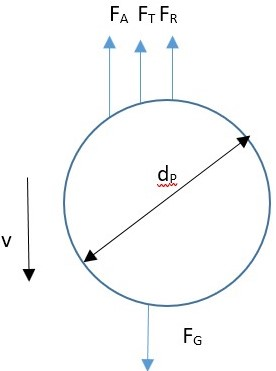
\includegraphics[width=0.22\textwidth]{img/partikelmodell}
	\caption{Skizze eines Partikels}
	\label{skizzepruef}
\end{figure}
\FloatBarrier
%Ende
\vspace*{-5mm}
\begin{flalign}
F_G &= m_P*g=V_P*\rho_P*g=\frac{\pi}{6}*d_P^3*\rho_P*g\\
F_T &= m_F*g=V_P*\rho_F*g=\frac{\pi}{6}*d_P^3*\rho_F*g
\end{flalign}
\begin{small}\begin{center}"'Auftrieb ist Masse der verdrängten Flüssigkeit"'\end{center}\end{small}
\vspace*{-5mm}
\begin{flalign}
F_R &= c_W*\rho_F*\frac{1}{2}*v_P^2*A_\perp
\end{flalign}


$c_W$... Widerstandsbeiwert $c_W=f(v,\text{Geometrie}, \text{Rauigkeit},...)$\\
$v_P$... Relativgeschwindigkeit zwischen Teilchen und Partikel\\
$A_\perp$... Projezierte Fläche des Partikels in Bewegungsrichtung\\
hier: Kugel $\rightarrow$ Kreis mit $A_\perp=\frac{\pi}{4}*d_P^2$















%Literaturverzeichnis Bücher
\bibliography{Literatur}
\bibliographystyle{unsrt}
\addcontentsline{toc}{chapter}{Literaturverzeichnis}

\begin{enumerate}
	\item Praktikumsskript, Modul ………, Versuch …….., Prof. Musterprof. 
	\item DIN 12345, Jahr der Veröffentlichung 
	\item Link der Internetseite, Zugriffsdatum 
	\item Buchtitel, Autor, Verlag, Veröffentlichungsjahr 
\end{enumerate}






%Anhang
\addcontentsline{toc}{chapter}{Anhang}

\end{document}
